\documentclass{article}
\usepackage[utf8]{inputenc}
\usepackage{subfig}
\usepackage{amsmath}
\usepackage[export]{adjustbox}
\usepackage{graphicx}
\usepackage[legalpaper, landscape, margin=0.5cm]{geometry}

\thispagestyle{empty}
% \renewcommand{\thesubfigure}{\roman{subfigure}}
\begin{document}

\begin{figure}[h]
        \centering
        \subfloat[typical lens casing]{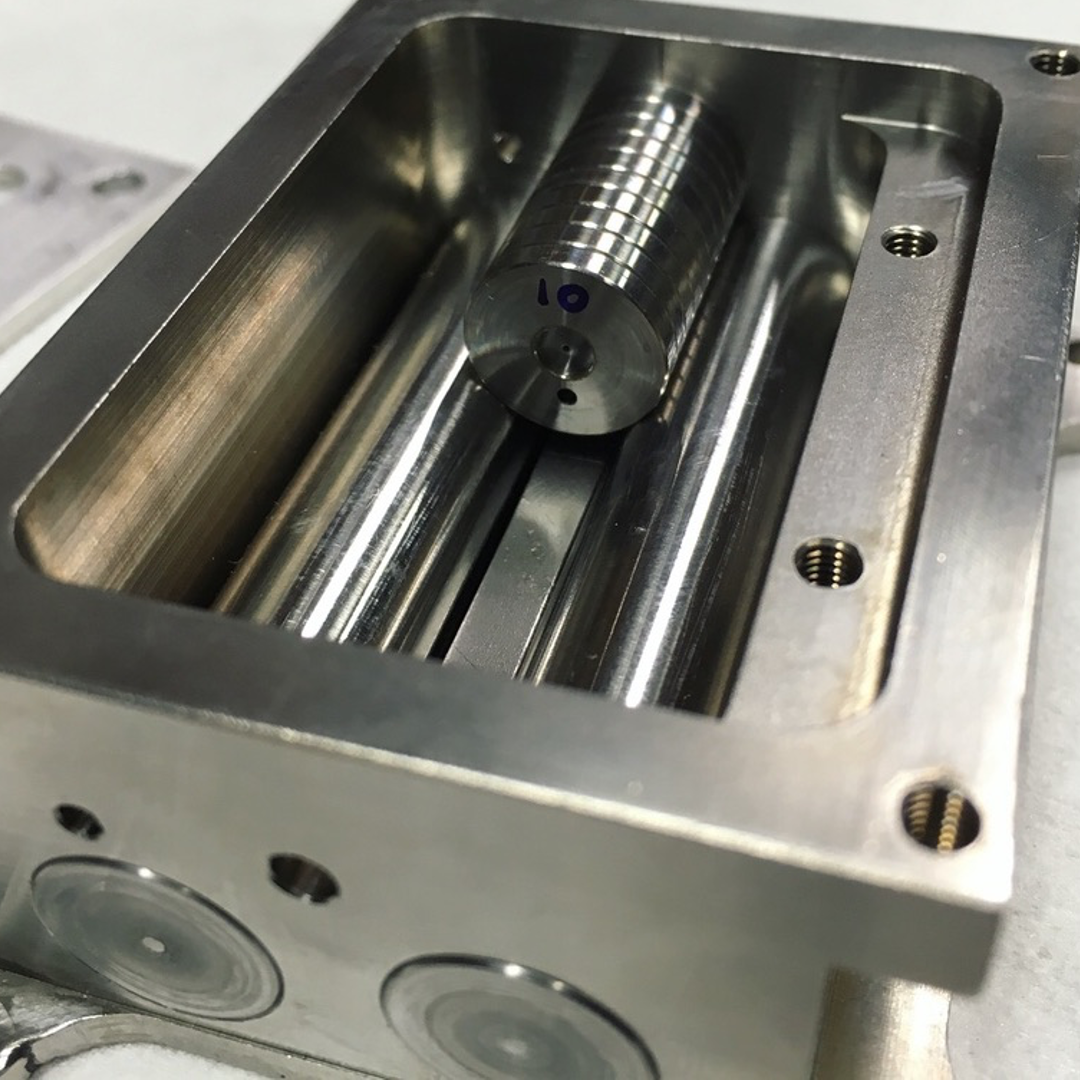
\includegraphics[height=4.3cm]{figures/ch06/ppr_01.png}}\hspace{0.1cm}
        \subfloat[lens in the frame]{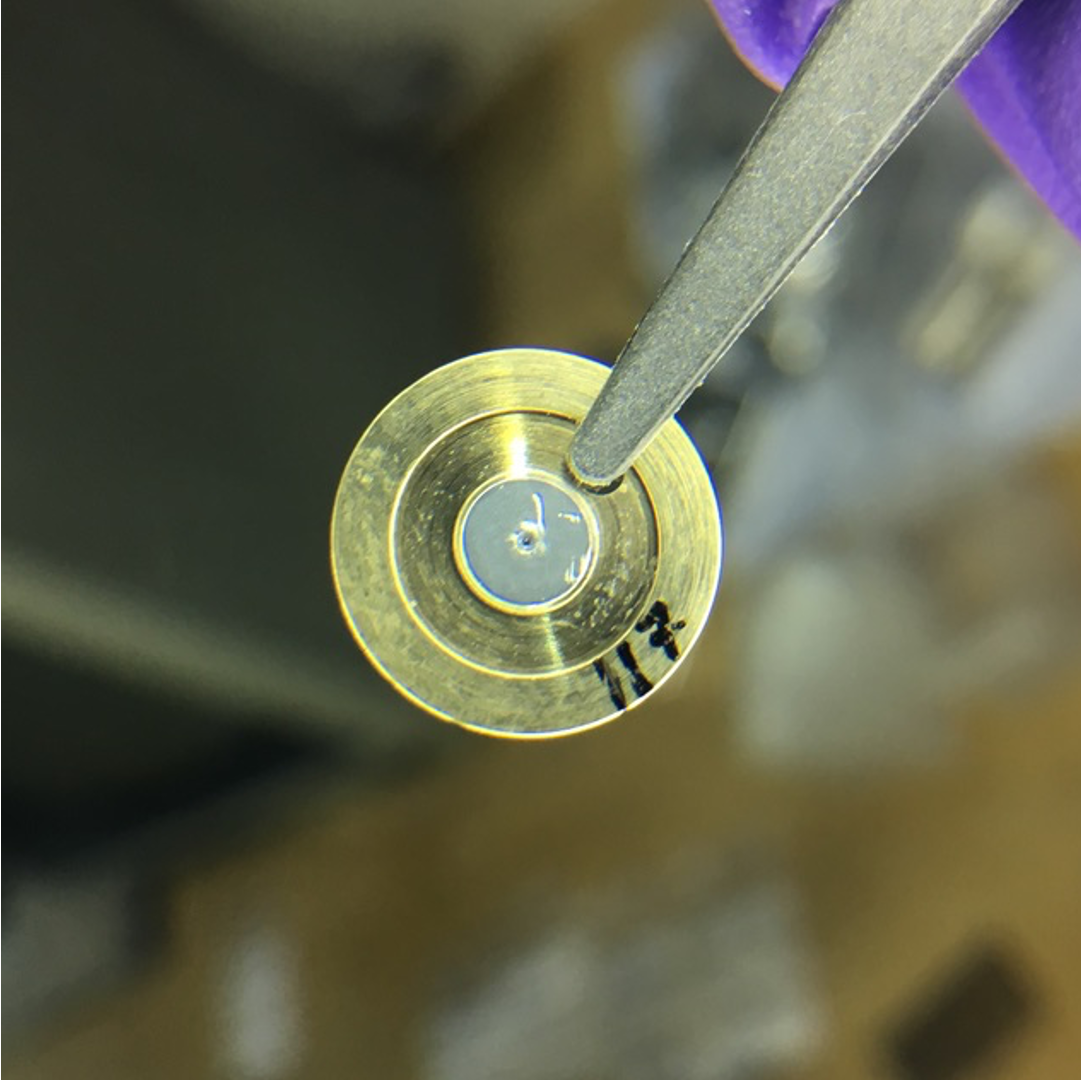
\includegraphics[height=4.3cm]{figures/ch06/ppr_02.png}}\hspace{0.1cm}
        \subfloat[1$^\text{st}$ gen. correction plate]{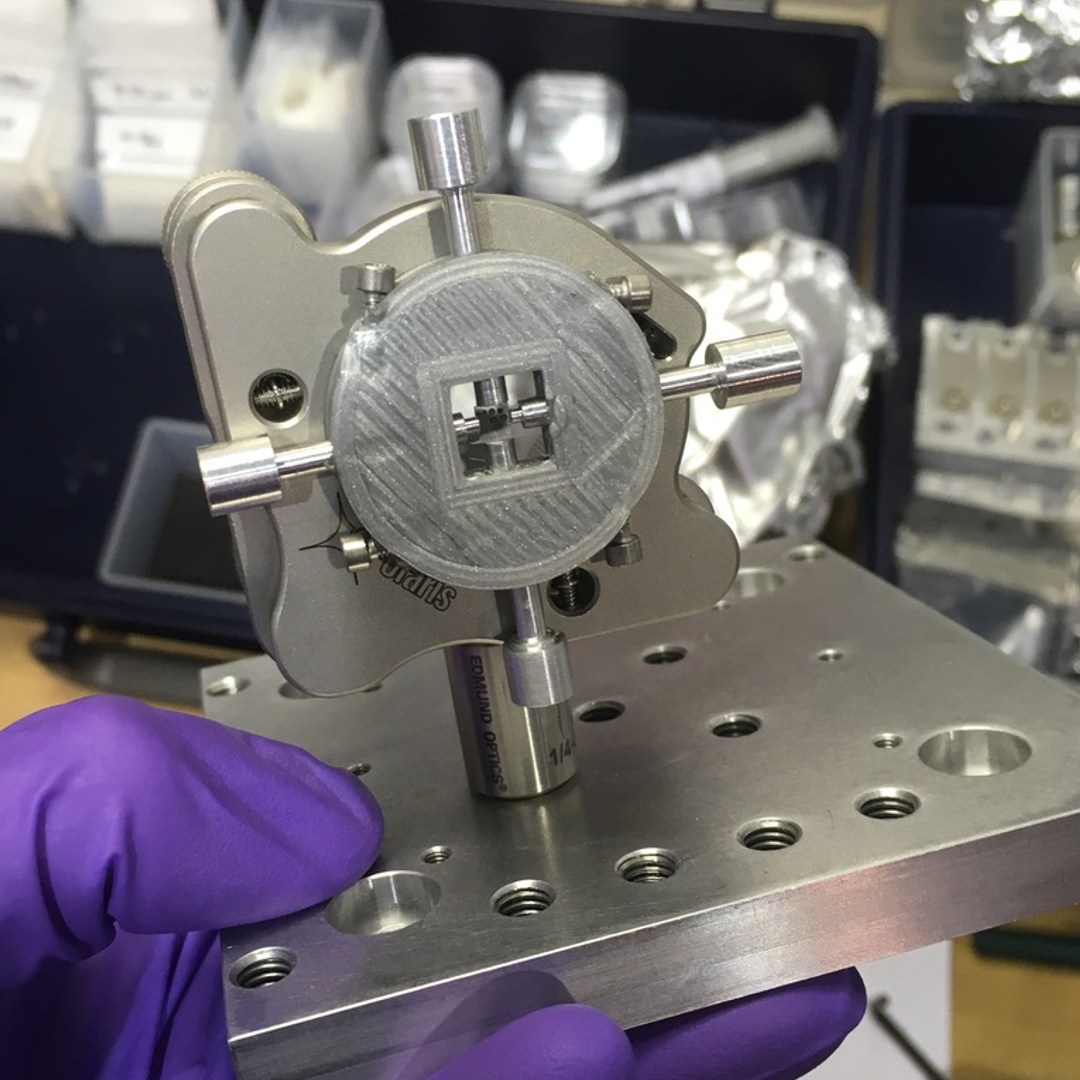
\includegraphics[height=4.3cm]{figures/ch06/ppr_03.png}}\hspace{0.1cm}
        \subfloat[2$^\text{nd}$ gen. correction plate]{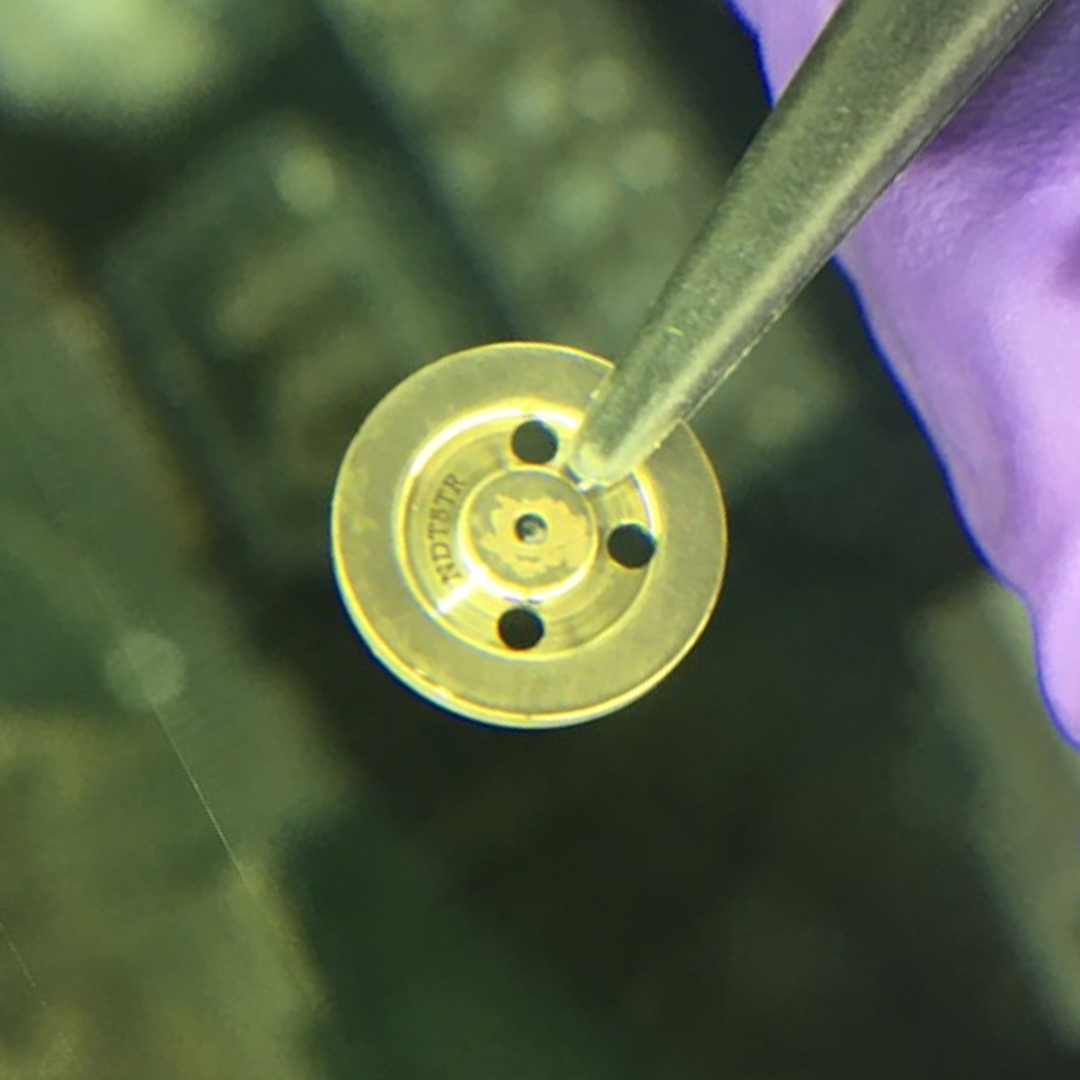
\includegraphics[height=4.3cm]{figures/ch06/ppr_04.png}}
 
\end{figure}
\end{document}